\section{El problema del viajante de comercio}

\begin{frame}{Problema}
Hallar el recorrido con distancia mínima en un conjunto de
ciudades que pase por todas las ciudades y regrese al punto inicial.

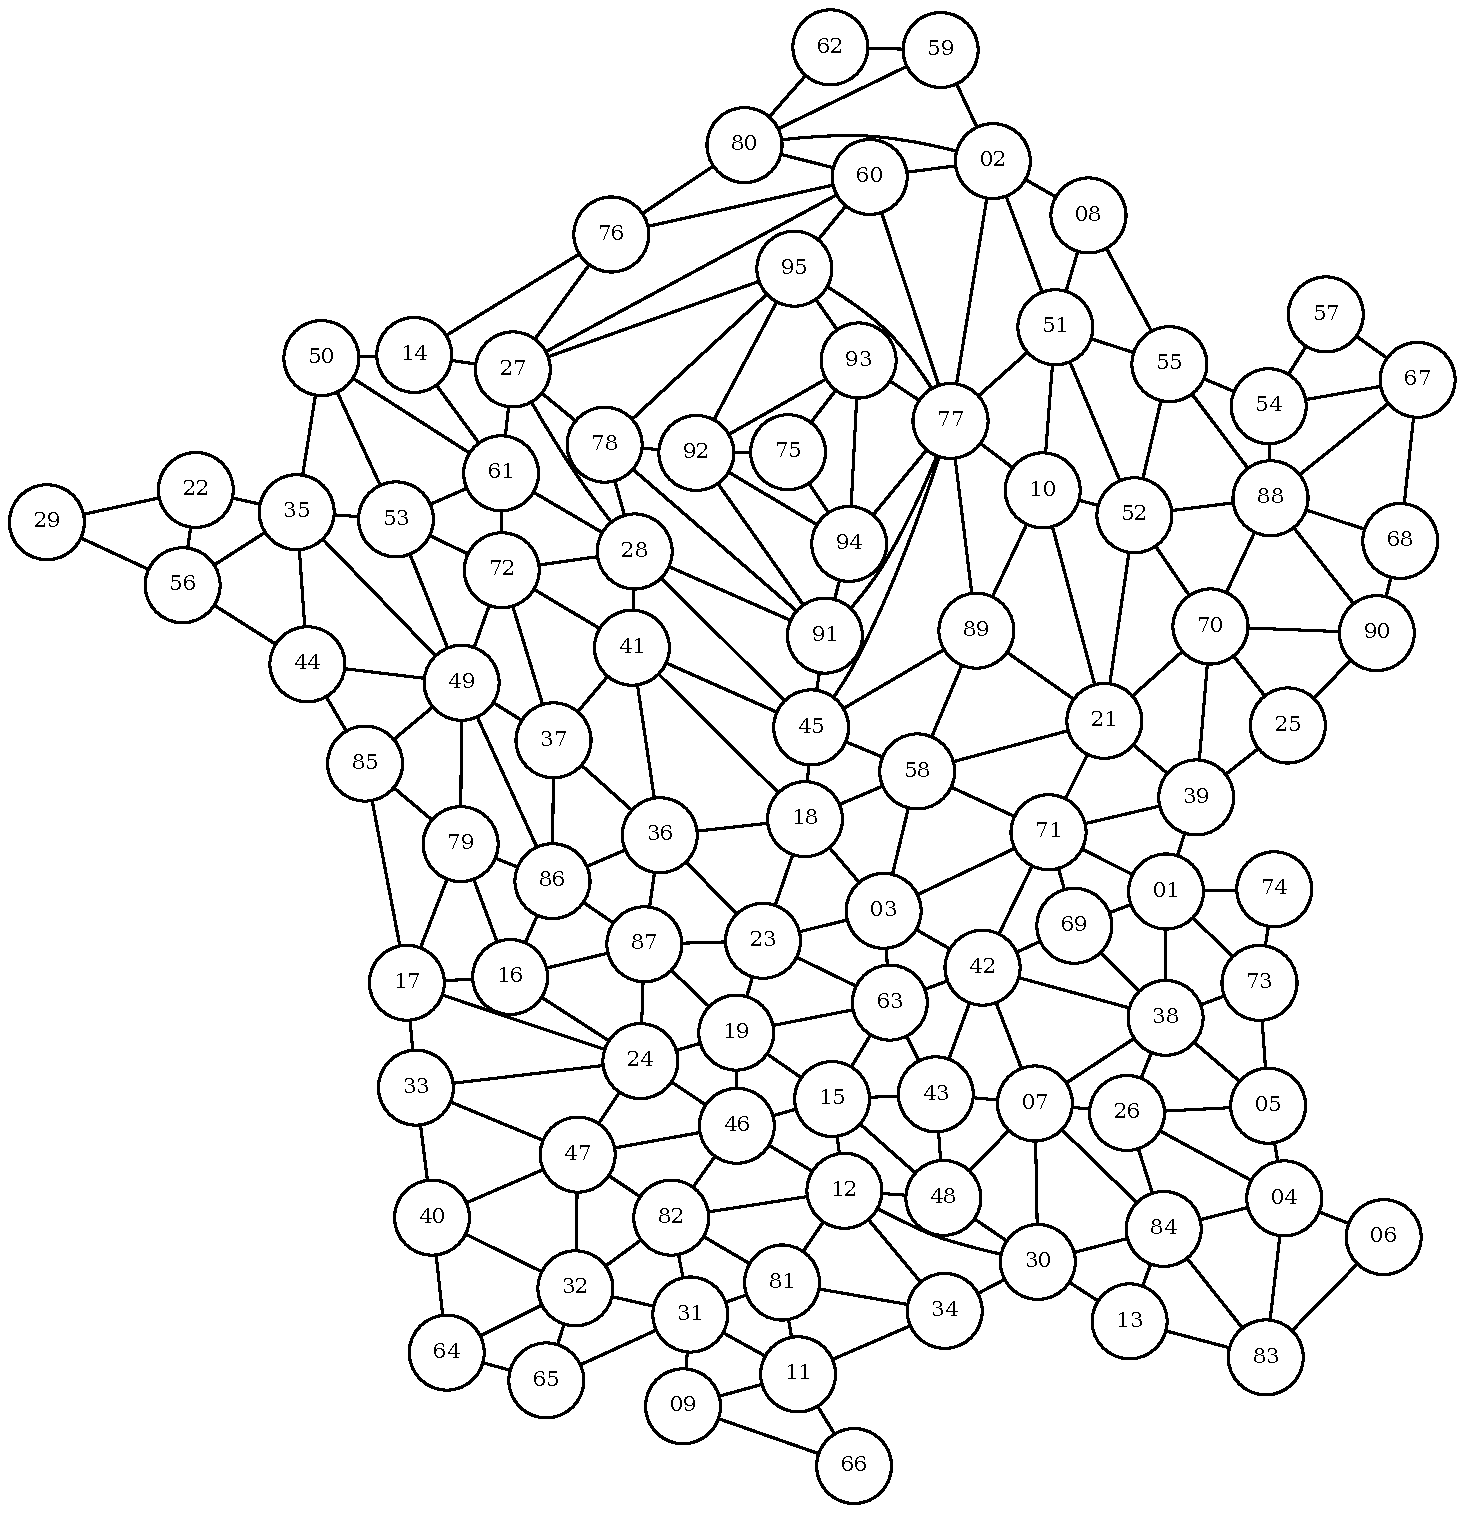
\includegraphics[width=.5\textwidth]{img/Francia} \centering
\end{frame}

\begin{frame}{Algoritmos}
\begin{description}
 \item[Entrada:] Ficheros con ciudades indicadas como puntos en el plano según sus
 coordenadas.
 \item[Salida:] \texttt{vector<int>} con el orden en el que se recorren las ciudades.
\end{description}
\end{frame}

\begin{frame}{Grafos}

Un grafo consta de:

\begin{itemize}
  \item Una \textbf{cantidad de nodos}, almacenada en el atributo \texttt{nodos}.
  \item Una \textbf{matriz de pesos}, almacenada en el vector \texttt{lados}.
\end{itemize}
\lstinputlisting[firstline=16, lastline=20]{cpps/grafo.h}
\end{frame}

\begin{frame}[fragile]{Construcción del grafo}
Construimos el grafo a partir de la distancia euclídea redondeada al entero más próximo.
\lstinputlisting[firstline=47, lastline=51]{cpps/grafo.h}
\end{frame}

\subsection{Algoritmos}

\begin{frame}[fragile]{Vecino más cercano}
Tomamos la ciudad inicial y almacenamos en las ciudades no visitadas:
\lstinputlisting[firstline=18, lastline=21]{cpps/tsp.cpp}
Devolveremos \texttt{trayecto}.
\end{frame}

\begin{frame}[fragile]{Vecino más cercano}
\vspace*{-.5cm}
Recorremos la lista buscando aquella ciudad con distancia mínima:
\lstinputlisting[firstline=23, lastline=37]{cpps/tsp.cpp}
\end{frame}

\begin{frame}{Inserción (algoritmo)}
  \begin{itemize}
    \item Toma como camino inicial los nodos más al norte, este y oeste
    \item Mientras haya nodos disponibles:
    \begin{itemize}
	    \item Para cada nodo disponible, halla la posición entre dos nodos del camino donde, de insertarse, se incrementaría menos la longitud del camino
	    \item Inserta el nodo que aumente menos la longitud en la posición que se calculó para ese nodo
    \end{itemize}
  \end{itemize}
\end{frame}

\begin{frame}[fragile]{Inserción (código)}
\vspace*{-.5cm}
\lstinputlisting[firstline = 95, lastline = 109]{cpps/tsp.cpp}
\end{frame}

\begin{frame}{Colonia de hormigas}
Este algoritmo se inspira en la comunicación por feromonas
de una colonia de hormigas para encontrar el camino mínimo hacia una fuente de comida.

\begin{center}
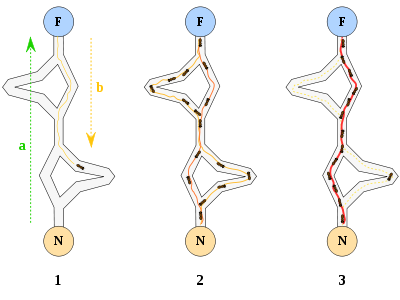
\includegraphics[width = 7cm ]{colonia_hormigas}
\end{center}

\end{frame}

\begin{frame}{Colonia}
Una Colonia consta de:
\begin{itemize}
  \item Grafo de \textbf{distancias} entre las ciudades.
  \item Grafo con las \textbf{feromonas} de cada camino, inicialmente arbitrarias.
  \item Constantes $\alpha, \beta, \rho, \xi, C, P, I$.
\end{itemize}
\note{Explicar qué son las feromonas}
\end{frame}

\begin{frame}{Constantes}
\begin{description}
  \item[$\alpha$] Peso que tienen las feromonas.
  \item[$\beta$] Peso que tienen la distancias.
  \item[$\rho$] Coeficiente de evaporación de las feromonas.
  \item[$\xi$] Coeficiente de debilitamiento de las feromonas.
  \item[$C$] Cuántas feromonas se añaden a un camino.
  \item[$P$] Probabilidad de tomar el camino más atractivo.
  \item[$I$] Cantidad de feromona inicial entre cada par de nodos.
\end{description}
\note{Explicar cada constante}
\end{frame}

\subsection{Ejemplos}
\begin{frame}{Comparativa de los algoritmos}
  A continuación ponemos tres ejemplos de ejecución de los algoritmos, para poder verlos y compararlos de una forma más eficaz.
  
  El tiempo de ejecución del algoritmo de colonia de hormigas es arbitrario y puede ajustarse a voluntad. A mayor tiempo de ejecución, mejor resultado ofrece. En general necesita más tiempo que los otros dos algoritmos para dar un resultado igual o mejor.
\end{frame}

\begin{frame}{Comparativa de longitudes}
	\begin{center}
		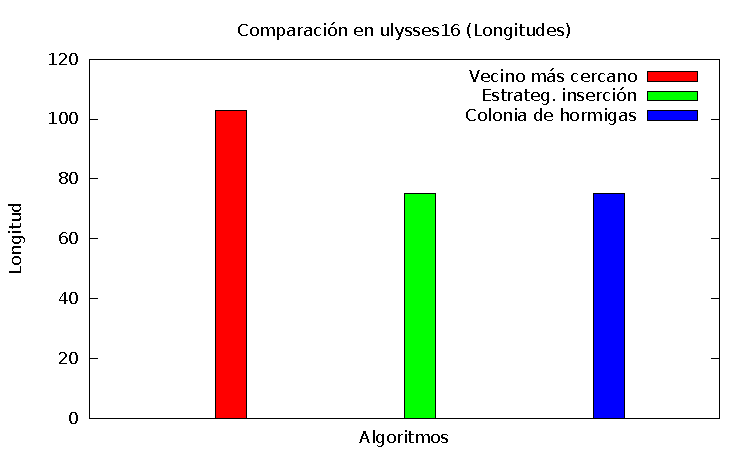
\includegraphics[width = \linewidth ]{barras_ulysses16_longitud}
	\end{center}
\end{frame}

\begin{frame}{Solución óptima}
\begin{center}
	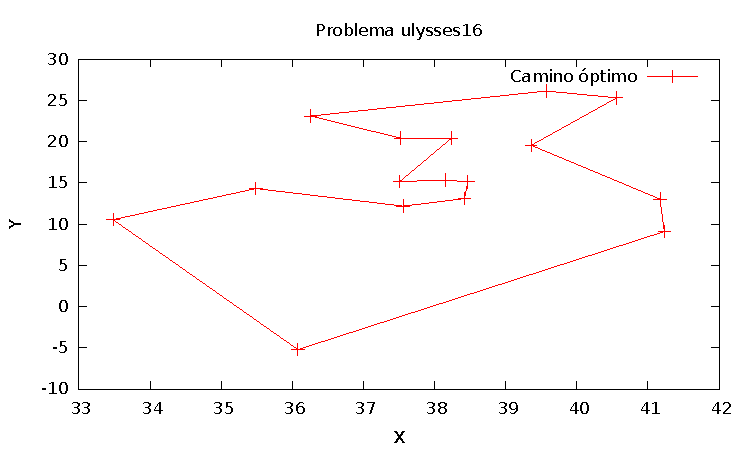
\includegraphics[width = \linewidth ]{ulysses16_tsp_opt}
\end{center}
\end{frame}

\begin{frame}{Solución de vecino más cercano}
	\begin{center}
		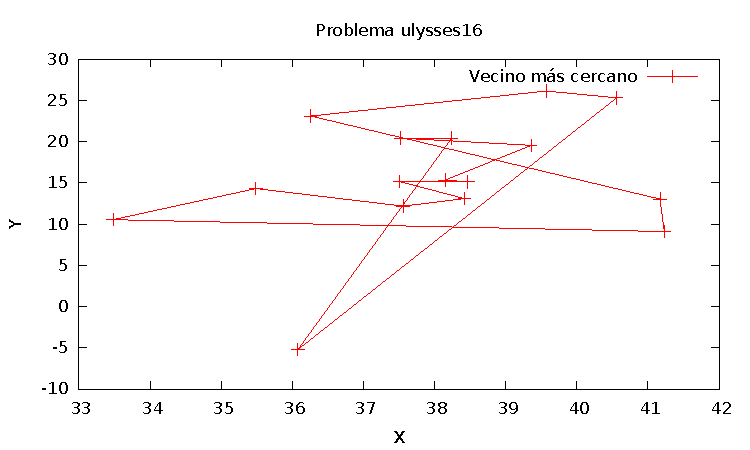
\includegraphics[width = \linewidth ]{ulysses16_tsp_1}
	\end{center}
\end{frame}

\begin{frame}{Solución de inserción}
	\begin{center}
		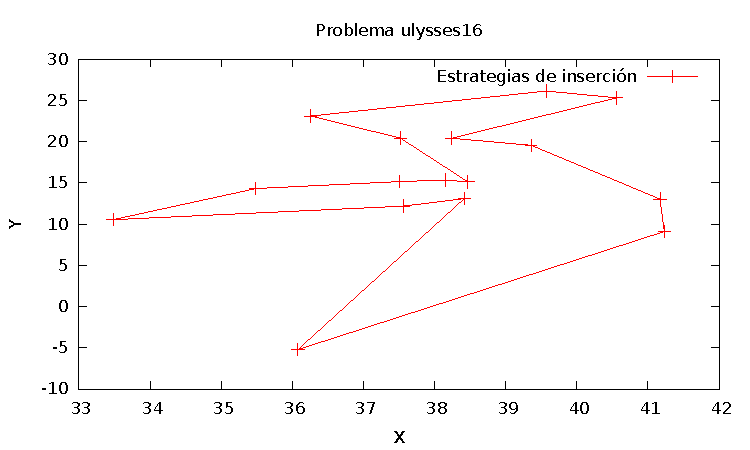
\includegraphics[width = \linewidth ]{ulysses16_tsp_2}
	\end{center}
\end{frame}

\begin{frame}{Solución de la colonia de hormigas}
	\begin{center}
		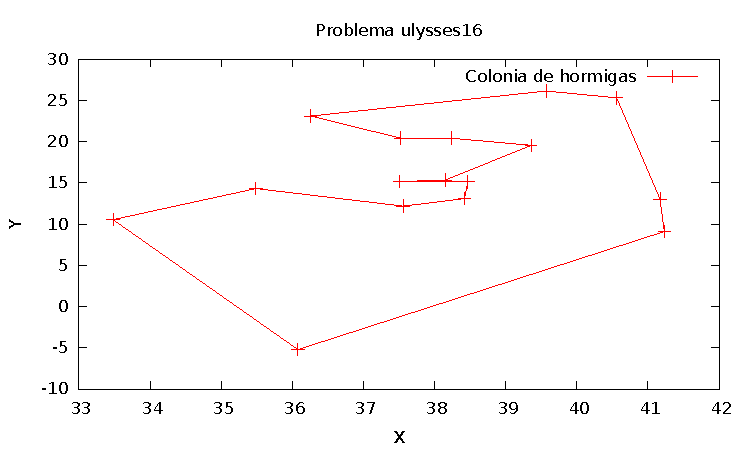
\includegraphics[width = \linewidth ]{ulysses16_tsp_3}
	\end{center}
\end{frame}

\begin{frame}{Comparativa de longitudes}
	\begin{center}
		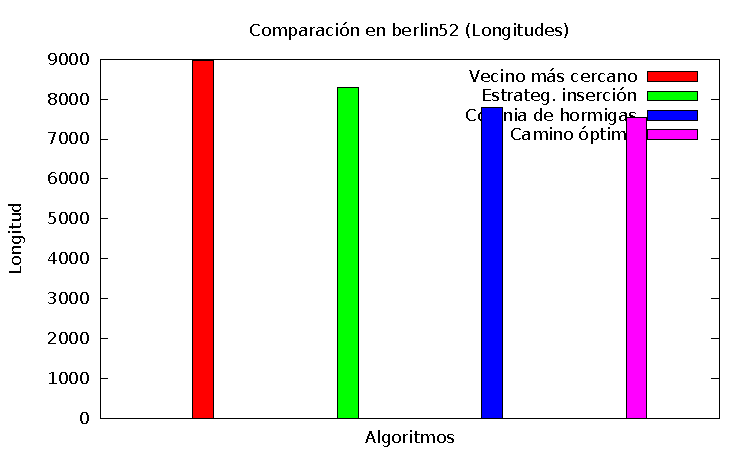
\includegraphics[width = \linewidth ]{barras_berlin52_longitud}
	\end{center}
\end{frame}

\begin{frame}{Solución óptima}
	\begin{center}
		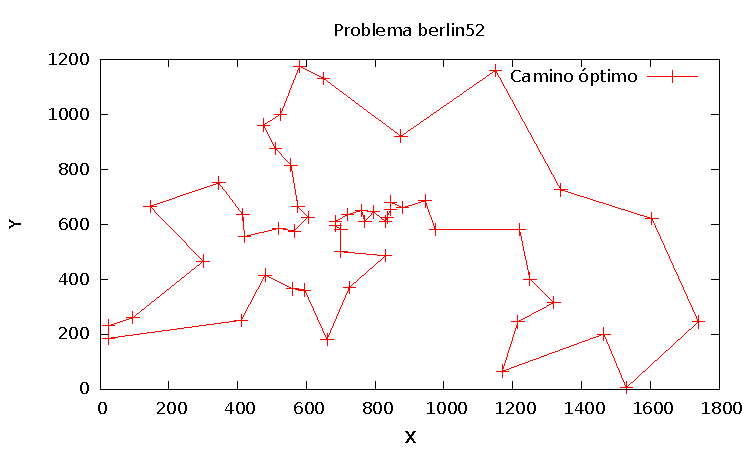
\includegraphics[width = \linewidth ]{berlin52_tsp_opt}
	\end{center}
\end{frame}

\begin{frame}{Solución de vecino más cercano}
	\begin{center}
		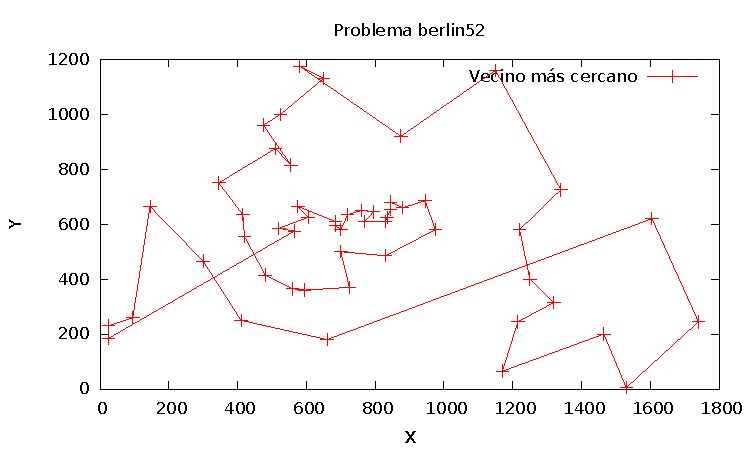
\includegraphics[width = \linewidth ]{berlin52_tsp_1}
	\end{center}
\end{frame}

\begin{frame}{Solución de inserción}
	\begin{center}
		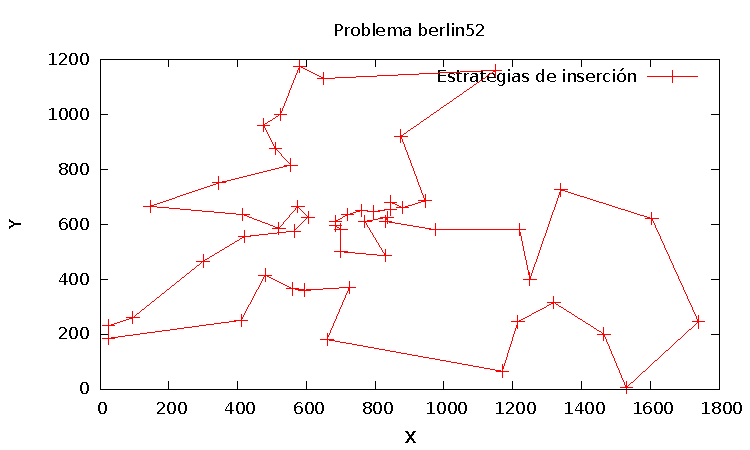
\includegraphics[width = \linewidth ]{berlin52_tsp_2}
	\end{center}
\end{frame}

\begin{frame}{Solución de la colonia de hormigas}
	\begin{center}
		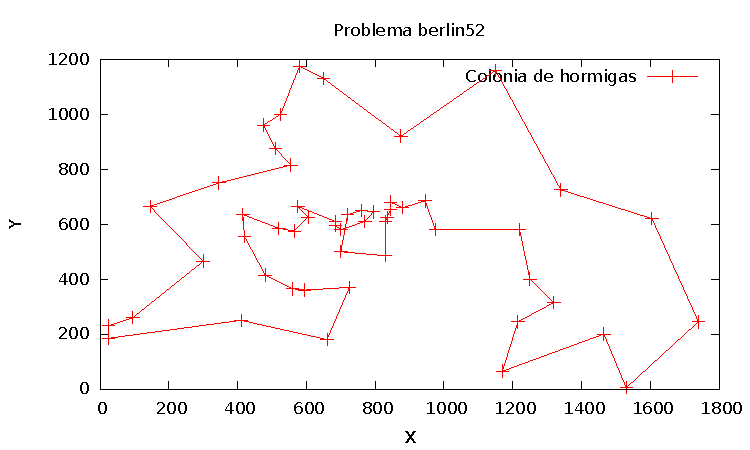
\includegraphics[width = \linewidth ]{berlin52_tsp_3}
	\end{center}
\end{frame}

\begin{frame}{Comparativa de longitudes}
	\begin{center}
		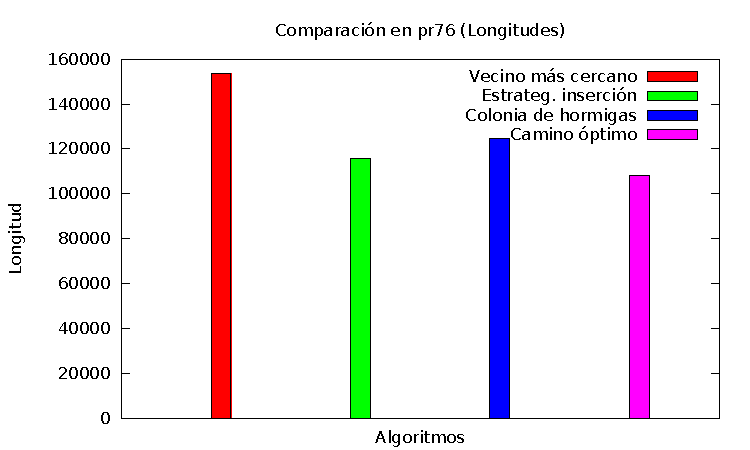
\includegraphics[width = \linewidth ]{barras_pr76_longitud}
	\end{center}
	\end{frame}

\begin{frame}{Solución óptima}
	\begin{center}
		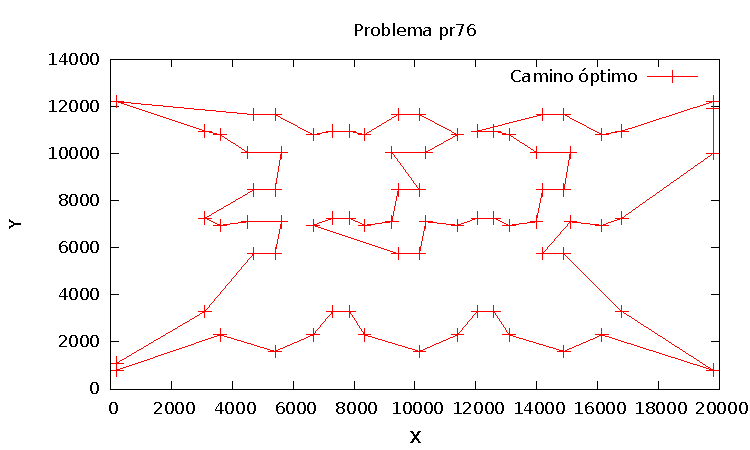
\includegraphics[width = \linewidth ]{pr76_tsp_opt}
	\end{center}
\end{frame}

\begin{frame}{Solución de vecino más cercano}
	\begin{center}
		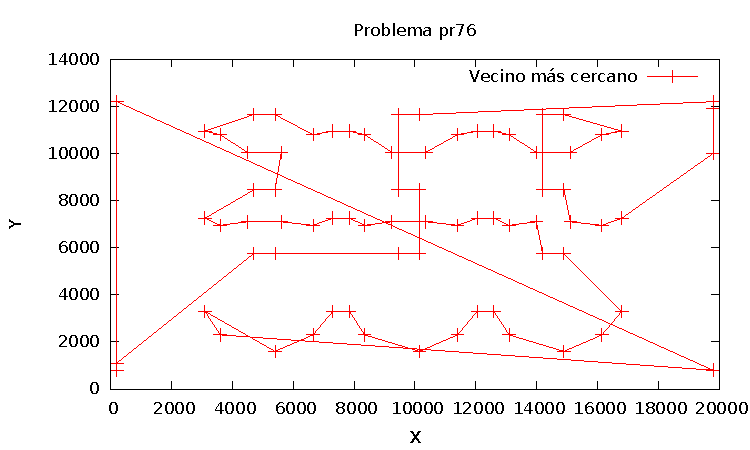
\includegraphics[width = \linewidth ]{pr76_tsp_1}
	\end{center}
\end{frame}

\begin{frame}{Solución de inserción}
	\begin{center}
		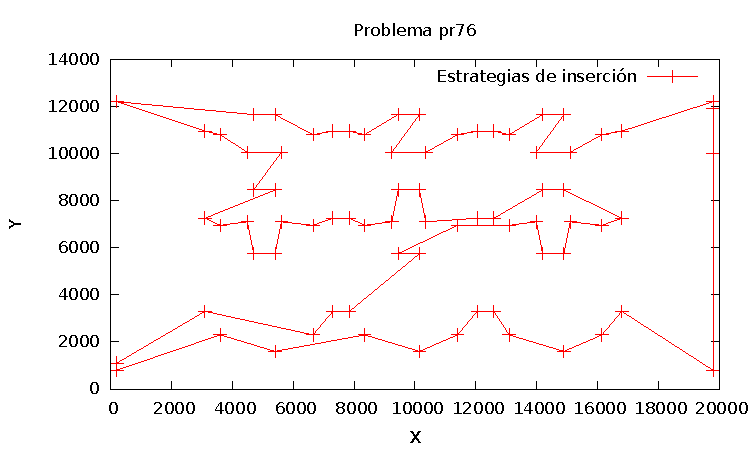
\includegraphics[width = \linewidth ]{pr76_tsp_2}
	\end{center}
\end{frame}

\begin{frame}{Solución de la colonia de hormigas}
	\begin{center}
		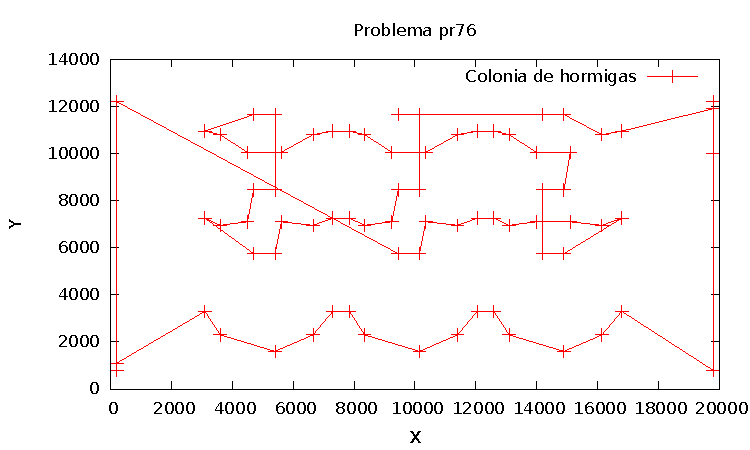
\includegraphics[width = \linewidth ]{pr76_tsp_3}
	\end{center}
\end{frame}
